\documentclass[../main.tex]{subfiles}

\begin{document}


\practica{Actualización remota (OTA) utilizando \emph{ThingsBoard}}

    \subsection{Objetivos}
        \begin{itemize}
            \item Entender la técnica de actualizaciones A/B.
            \item Preparar una aplicación para que sea actualizable.
            \item Comprender el funcionamiento de los bits de opción de arranque del procesador.
        \end{itemize}

    \subsection{Fundamentos teóricos}

        Aunque los sistemas empotrados suelen tener funciones muy específicas y constantes a lo largo del tiempo, su complejidad a día de hoy hace que, en ocasiones, se cuele algún bug, o haga falta realizar algún cambio en los programas que los gobiernan. 

        Cuando desarrollamos desde nuestro ordenador, con un cable conectado, este proceso es muy sencillo: con un depurador (bien externo o integrado en la placa) podemos cambiar el código fácilmente. Sin embargo, al desplegar las soluciones en el mundo real, perdemos el acceso directo. Únicamente el propio controlador, a través de las interfaces que lo conecten al mundo exterior, es capaz de recibir información y, potencialmente, actualizarse.

        Existen numerosas maneras de realizar estas actualizaciones remotas, aunque todas tienen algo en común: El código que actualiza la aplicación, no puede actualizarse a sí mismo, o de lo contrario se puede corromper mientras se actualiza. Para salvar esta barrera, existen numerosas técnicas, por ejemplo utilizando \emph{bootloaders}, utilizando \emph{launchers} con la única función de actualizar, haciendo que la propia app se actualice...

        En nuestro caso vamos a utilizar una de las aproximaciones más robustas ante fallos, conocida como las actualizaciones A/B. En esta aproximación, se divide el espacio de memoria en dos zonas (A y B), de tal manera que la aplicación pueda residir en ambas. Cuando la app aranca desde A, en caso de encontrar una actualización la hará en B, y viceversa. Los bits de arranque del sistema se configuran, en cada caso, para arrancar la app más nueva. Añadiendo pasos de comprobación de integridad de los datos, se asegura, antes de cambiar el arranque, que la aplicación descargada no tiene fallos. Con todo esto, las probabilidades de \emph{brickear} (o dejar inutilizable) el dispositivo se reducen enormemente. Este flujo general puede verse en \Cref{fig:a_b_update}.

        \begin{figure}
            \begin{tikzpicture}[
                font=\sffamily,
                % Core component styles
                mcu/.style={draw, thick, rectangle, rounded corners, fill=gray!10, minimum width=3.0cm, minimum height=1.3cm, align=center},
                flash/.style={draw, thick, rectangle, fill=white, minimum width=3.2cm, minimum height=4.6cm},
                slot/.style={draw, thick, rectangle, minimum height=1.1cm, minimum width=2.8cm, align=center, inner sep=3pt, font=\small},
                active_app/.style={fill=blue!15, draw=blue!80!black},
                inactive_app/.style={fill=gray!20, draw=gray!50},
                new_app/.style={fill=green!15, draw=green!70!black},
                broker/.style={draw, thick, ellipse, fill=orange!15, draw=orange!80!black, minimum width=2.4cm, minimum height=1.0cm, align=center, font=\small},
                % Arrow styles
                arrow_std/.style={-{Stealth[scale=0.9]}, thick},
                arrow_flash/.style={-{Stealth[scale=0.9]}, thick, red!70!black},
                arrow_mqtt/.style={-{Stealth[scale=0.9]}, thick, orange!70!black, dashed},
                label_txt/.style={font=\sffamily\tiny\bfseries, align=center},
                phase_box/.style={draw=gray!40, fill=gray!2, dashed, rounded corners=8pt, inner sep=12pt}
            ]

                % Coordinates for 4 Phase Centers (Clockwise Grid Layout)
                \coordinate (P1) at (0, 0);        % Top-Left: Phase 1
                \coordinate (P2) at (9, 0);     % Top-Right: Phase 2
                \coordinate (P3) at (9, -9);  % Bottom-Right: Phase 3
                \coordinate (P4) at (0, -9);     % Bottom-Left: Phase 4

                % ==============================================================================
                % PHASE 1: Normal Operation (App A Active)
                % ==============================================================================
                \node[font=\bfseries\large] (t1) at ($(P1)+(0,3.6)$) {1. Startup (App A Active)};
                \node[mcu] (mcu1) at ($(P1)+(-2.0,-0.8)$) {\textbf{MCU}\\Running App A};
                \node[font=\scriptsize\bfseries, text=blue!80!black, below= 2pt of mcu1] {VTOR $\to$ 0x08000000};

                \node[flash] (f1) at ($(P1)+(2.0,-0.2)$) {};
                \node[font=\bfseries\small, above=-0.1cm of f1.north] {Flash Memory};
                \node[slot, inactive_app] (f1_boot) at ($(P1)+(2.0,1.3)$) {\textbf{Boot Bytes}\\Points to A};
                \node[slot, active_app] (f1_slota) at ($(P1)+(2.0, -0.1)$) {\textbf{Slot A} \\ (0x08000000)\\Running V1};
                \node[slot, inactive_app] (f1_slotb) at ($(P1)+(2.0, -1.5)$) {\textbf{Slot B} \\ (0x08040000)\\Old / Empty};

                \draw[arrow_std] (f1_boot.west) -| node[pos=0.5, above, font=\tiny] {Initial Boot} (mcu1.north);

                % ==============================================================================
                % PHASE 2: Update Received & Flashed
                % ==============================================================================
                \node[font=\bfseries\large] (t2) at ($(P2)+(0,3.6)$) {2. Update Received \& Flashed};
                \node[broker] (br2) at ($(P2)+(-2.0,1.8)$) {\textbf{MQTT}\\Broker};
                \node[mcu] (mcu2) at ($(P2)+(-2.0,-0.8)$) {\textbf{MCU}\\Running App A};

                \node[flash] (f2) at ($(P2)+(2.0,-0.2)$) {};
                \node[font=\bfseries\small, above=-0.1cm of f2.north] {Flash Memory};
                \node[slot, inactive_app] (f2_boot) at ($(P2)+(2.0,1.3)$) {\textbf{Boot Bytes}\\Points to A};
                \node[slot, active_app] (f2_slota) at ($(P2)+(2.0, -0.1)$) {\textbf{Slot A} \\ (0x08000000)\\Downloading...};
                \node[slot, new_app] (f2_slotb) at ($(P2)+(2.0, -1.5)$) {\textbf{Slot B} \\ (0x08040000)\\Flashing V2...};

                \draw[arrow_mqtt, <-] (mcu2.north) -- (br2.south) node[midway, right, label_txt] {Download\\App V2};
                \draw[arrow_flash] (mcu2.east) -- (f2_slotb.west) node[midway, below, label_txt, text=red!70!black] {Write \\ Image};

                % ==============================================================================
                % PHASE 3: Configure Boot Switch
                % ==============================================================================
                \node[font=\bfseries\large] (t3) at ($(P3)+(0,3.6)$) {3. Configure Boot Switch};
                \node[mcu] (mcu3) at ($(P3)+(-2.0,-0.8)$) {\textbf{MCU}\\Running App A};

                \node[flash] (f3) at ($(P3)+(2.0,-0.2)$) {};
                \node[font=\bfseries\small, above=-0.1cm of f3.north] {Flash Memory};
                \node[slot, new_app] (f3_boot) at ($(P3)+(2.0,1.3)$) {\textbf{Boot Bytes}\\Update to B};
                \node[slot, active_app] (f3_slota) at ($(P3)+(2.0, -0.1)$) {\textbf{Slot A} \\ (0x08000000)\\Finalizing...};
                \node[slot, new_app] (f3_slotb) at ($(P3)+(2.0, -1.5)$) {\textbf{Slot B} \\ (0x08040000)\\V2 Verified};

                \draw[arrow_flash] (mcu3.north) |- (f3_boot.west) node[pos=0.7, above, label_txt, text=red!70!black] {1. Set Boot Flag};
                \draw[arrow_std, red!70!black] (mcu3.south) -- ++(0,-0.4) node[below, label_txt, text=red!70!black] {2. System Reset};

                % ==============================================================================
                % PHASE 4: Post-Update Operation (App B Active)
                % ==============================================================================
                \node[font=\bfseries\large] (t4) at ($(P4)+(0,3.6)$) {4. Post-Update (App B Active)};
                \node[mcu] (mcu4) at ($(P4)+(-2.0,-0.8)$) {\textbf{MCU}\\Running App B};
                \node[font=\scriptsize\bfseries, text=green!70!black, below= 2pt of mcu4] {VTOR $\to$ 0x08040000};

                \node[flash] (f4) at ($(P4)+(2.0,-0.2)$) {};
                \node[font=\bfseries\small, above=-0.1cm of f4.north] {Flash Memory};
                \node[slot, active_app] (f4_boot) at ($(P4)+(2.0,1.3)$) {\textbf{Boot Bytes}\\Points to B};
                \node[slot, inactive_app] (f4_slota) at ($(P4)+(2.0, -0.1)$) {\textbf{Slot A} \\ (0x08000000)\\Old V1};
                \node[slot, active_app] (f4_slotb) at ($(P4)+(2.0, -1.5)$) {\textbf{Slot B} \\ (0x08040000)\\Running V2};

                \draw[arrow_std] (f4_boot.west) -| node[pos=0.5, above, font=\tiny] {New Boot} (mcu4.north);

                % ==============================================================================
                % BACKGROUND BOXES & PROCESS FLOW ARROWS
                % ==============================================================================
                \begin{pgfonlayer}{background}
                    \node[phase_box, fit=(t1) (mcu1) (f1) (f1_boot) (f1_slotb)] (box1) {};
                    \node[phase_box, fit=(t2) (br2) (mcu2) (f2) (f2_boot) (f2_slotb)] (box2) {};
                    \node[phase_box, fit=(t3) (mcu3) (f3) (f3_boot) (f3_slotb)] (box3) {};
                    \node[phase_box, fit=(t4) (mcu4) (f4) (f4_boot) (f4_slotb)] (box4) {};

                    % Clockwise flow arrows connecting phases
                    \draw[-{Stealth[scale=1.2]}, line width=1.5pt, gray!70] (box1.east) -- (box2.west);
                    \draw[-{Stealth[scale=1.2]}, line width=1.5pt, gray!70] (box2.south) -- (box3.north);
                    \draw[-{Stealth[scale=1.2]}, line width=1.5pt, gray!70] (box3.west) -- (box4.east);
                    \draw[-{Stealth[scale=1.2]}, line width=1.5pt, gray!70] (box4.north) -- (box1.south)
                        node[midway, fill=white, inner sep=3pt, font=\sffamily\small\bfseries, text=gray!80!black] {Reciprocal Process (App B updates App A)};
                \end{pgfonlayer}
            \end{tikzpicture}
            \caption{Diagrama de actualización A/B}
            \label{fig:a_b_update}
        \end{figure}

        \subsubsection{El problema de la compilación}
            
            Al compilar una aplicación para un sistema empotrado, normalmente se prepara con la idea de que siempre va a arrancar desde el mismo espacio en la memoria. De hecho, el código, en general no es de tipo PIC (position independent code), sino que ciertas direcciones de memoria están fijadas y no pueden cambiar. Al aplicar esta división A/B, esto sería un problema: la aplicación arranca desde dos direcciones de memoria diferentes. Es por ello que, en este tipo de aplicaciones, hay varias cosas a tener en cuenta:

            \begin{itemize}
                \item La aplicación debe ser consciente de cuál es su dirección de arranque (A o B).
                \item Se deben realizar dos compilaciones diferentes (A y B), cada una atacando una de las dos regiones de memoria. 
                \item Cada compilación sólo puede residir en su zona de compilación predeterminada, con lo cual el sistema de actualizaciones deberá tenerlo en cuenta.
            \end{itemize}

    \subsection{Desarrollo de la práctica}

        \subsubsection{Preparación del código}

            El código ya está preparado para descargar la actualización OTA de \emph{ThingsBoard} (configuraremos la interfaz web más adelante). Explicamos aquí con detalle los cambios respecto a la anterior práctica.

            En la función \texttt{ESP01S\_ProcessMQTT} tenemos los primeros cambios. En primer lugar, observamos que, además de comprobar en los mensajes de entrada las cadenas de actualización de \texttt{ledState}, ahora se llama a la función \texttt{OTA\_ProcessJSON}. Está función (definida en los nuevos archivos \texttt{ota.h} y \texttt{ota.c}) se encarga de parsear el aviso de nuevo firmware disponible desde el servidor. Adicionalmente, se añade una comprobación directa para mensajes recibidos con el propio firmare (a través del \emph{topic} \textbf{MQTT} ``v2/fw/response'').

            \begin{lstlisting}
                if (MQTTDeserialize_publish(&dup, &qos, &retained, NULL, &receivedTopic,
                                            &payload, &payloadlen, packet, copy_len) == 1)
                {
                    //Debug_Printf("[MQTT RX] %s\r\n", receivedTopic.lenstring.data);
                    // 1. Handle Binary Firmware Response Chunk
                    if (memcmp(receivedTopic.lenstring.data, "v2/fw/response", 14) == 0 && OTA_getState() == OTA_STATE_DOWNLOADING) {
                        OTA_WriteChunkAndProcess(payload, payloadlen);
                    }
                    // 2. Handle JSON Attributes (Runtime Notification or Startup Request)
                    else {
                        char json_str[128] = {0};
                        uint16_t str_len = (payloadlen < sizeof(json_str) - 1) ? payloadlen : sizeof(json_str) - 1;
                        memcpy(json_str, payload, str_len);

                        OTA_ProcessJSON(json_str);

                        // LED command processing
                        if (strstr(json_str, "\"ledState\":true"))        GPIO_PIN_WRITE(GPIOA, 7, GPIO_STATE_ONE);
                        else if (strstr(json_str, "\"ledState\":false"))   GPIO_PIN_WRITE(GPIOA, 7, GPIO_STATE_ZERO);
                    }
                }
            \end{lstlisting}

            Para estar en el modo de descarga de firmware, primero este debe ser solicitado. La función \texttt{OTA\_ProcessJSON} se encarga de extraer la versión y tamaño del firmware anunciado desde el servidor. La versión desde el servidor tendrá la forma \texttt{1.0.0\_A} o \texttt{1.0.0\_B}, según el \emph{slot} que ocupe. Esto sirve para identificar dos cosas: en primer lugar, si la versión es superior a la actual (definida en \texttt{ota.h} como \lstinline|#define CURRENT_FW_VERSION "1.0.0"|), y si es la adecuada para el \emph{slot} libre. En tal caso, se procede a borrar los sectores adecuados de la \PER{FLASH}, y a solicitar los \emph{chunks} o trozos de actualización uno tras otro (ya que, en general, las actualizaciones son demasiado grandes como para descargarlas de golpe).

            \begin{lstlisting}
                void OTA_ProcessJSON(const char *json) {
                    char *ver_ptr = strstr(json, "\"fw_version\":");
                    char *size_ptr = strstr(json, "\"fw_size\":");

                    if (ver_ptr && size_ptr && ota_ctx.state == OTA_STATE_IDLE) {
                        char new_version[32] = {0};
                        sscanf(ver_ptr, "\"fw_version\":\"%31[^\"]\"", new_version);
                        uint32_t new_size = (uint32_t)atoi(size_ptr + 10);

                        // Determine what binary suffix this device requires
                        const char *required_suffix = ((uint32_t)&_app_start == FLASH_SLOT_A_ADDR) ? "B" : "A";

                        // Reject the update if the incoming version tag doesn't match the inactive slot
                        if (strstr(new_version, required_suffix) == NULL) {
                            Debug_Printf("[OTA] Rejected update %s! Device is running in Slot %c and requires %s binary.\r\n",
                                        new_version,
                                        ((uint32_t)&_app_start == FLASH_SLOT_A_ADDR) ? 'A' : 'B',
                                        required_suffix);
                            return;
                        }

                        // Verify if version differs from running app
                        if (strcmp(new_version, CURRENT_FW_VERSION) != 0 && new_size > 0) {
                            Debug_Printf("[OTA] New Version Found: %s (Size: %lu bytes)\r\n", new_version, new_size);

                            ota_ctx.state = OTA_STATE_DOWNLOADING;
                            ota_ctx.total_size = new_size;
                            ota_ctx.bytes_downloaded = 0;
                            ota_ctx.current_chunk = 0;
                            strncpy(ota_ctx.target_version, new_version, sizeof(ota_ctx.target_version));

                            OTA_EraseTargetSlot();
                            OTA_RequestNextChunk();
                        }
                    }
                }
            \end{lstlisting}

            Estos \emph{chunks} se van procesando en \texttt{OTA\_WriteChunkAndProcess}. Esta función va situando el puntero de escritura de la \PER{FLASH} para ir poco a poco escribiendo el nuevo firmware, hasta completar la descarga. 

            \begin{lstlisting}
                void OTA_WriteChunkAndProcess(uint8_t *data, uint16_t length) {
                    OTA_WriteChunk(ota_ctx.bytes_downloaded, data, length);
                    ota_ctx.bytes_downloaded += length;
                    ota_ctx.current_chunk++;

                    Debug_Printf("[OTA RX] Chunk %u (%d bytes) -> Total: %lu / %lu\r\n",
                                ota_ctx.current_chunk, length, ota_ctx.bytes_downloaded, ota_ctx.total_size);

                    if (ota_ctx.bytes_downloaded < ota_ctx.total_size) {
                        OTA_RequestNextChunk();
                    } else {
                        Debug_Printf("[OTA SUCCESS] Download Finished! Rebooting...\r\n");
                        ota_ctx.state = OTA_STATE_COMPLETE;
                        OTA_SwapBootSlotAndReset();
                    }
                }
            \end{lstlisting}

            Cuando la descarga está completa, se lanza \texttt{OTA\_SwapBootSlotAndReset}. Esta función tiene la importante función de calcular la nueva dirección de arranque y grabarla en los bits de opción (\REFMAN[3.4.1]), para que la siguiente vez que el procesador comience, lo haga desde el nuevo \emph{slot}. Los bits de opción de la \PER{FLASH} permiten precisamente configurar ciertas opciones de arranque, que son tenidas en cuenta antes de que comience a ejecutar cualquier código. Así, no es la aplicación quién decide desde qué dirección se arranca, sino el propio procesador.

            En nusetro procesador \MCU, existen dos posibles direcciones de arranque \REFMAN[3.7.7]. El hecho de existir dos es para dar la opción de, al resetear, elegir cuál sirve de arranque con la pulsación (o no) de un botón. Normalmente, lo que se hace es colocar un \emph{bootloader} en una de las direcciones iniciales, y nuestra aplicación en la otra. Esto hará que, si por algún motivo nuestra aplicación está mal escrita y no tiene comunicación con el depurador, se pueda recuperar la misma cargando el \emph{bootloader}. En nuestra placa, al tener un depurador integrado, no tenemos que preocuparnos de ningún problema, ya que el depurador está conectado directamente por un puerto \texttt{SWI} (Serial Wire Interface) que puede tomar el control total del procesador aunque se quede ``pillado''. 

            En resumen, lo que haremos será ajustar la dirección \texttt{BOOT\_ADD0} en \REG{OPTCR1} para apuntar a la aplicación que queramos arrancar. Como estos bits son delicados, no se puede escribir directamente en ellos, y hay que aplicar una secuencia de desbloqueo a través de los registros \REG{CR} (\REFMAN[3.7.5]), \REG{KEYR} (\REFMAN[3.7.2]), \REG{OPTCR} (\REFMAN[3.7.6]) y \REG{OPTKEYR} (\REFMAN[3.7.3]). Tras hacerlo, forzamos un volcado de la memoria mediante la primitiva \texttt{\_\_DSB()}, y reseteamos el sistema desde el \REG{AIRCR} del \PER{SCB} (\PMMAN[4.3.5]).

            \begin{lstlisting}
                void OTA_SwapBootSlotAndReset(void)
                {
                    uint32_t target_addr = OTA_GetTargetAddress();
                    // BOOT_ADD0 expects the flash address divided by 16KB (shifted right by 14 bits)
                    uint16_t boot_val = (uint16_t)(target_addr >> 14);

                    Debug_Printf("[OTA] Swapping BOOT_ADD0 to 0x%08LU (val: 0x%04X) and resetting...\r\n",
                                target_addr, boot_val);
                    Delay_ms(500);

                    Flash_Unlock(); // Uses bsp.h helper
                    Flash_Unlock_Opt();
                    Flash_WaitNotBusy(); // Uses bsp.h helper

                    //update target boot address
                    Flash_Update_Opt(boot_val);

                    Flash_WaitNotBusy();
                    Flash_Lock_Opt();
                    Flash_Lock(); // Uses bsp.h helper

                    // Force system reset after Data Syncrhonization Barrier
                    // (to flush pending mem stores)
                    __DSB();
                    SCB->AIRCR = (0x05FA0000U) | (1U << 2); // VECTKEY (0x05FA) + SYSRESETREQ (Bit 2)

                    while (1); // Wait for hardware reset
                }
            \end{lstlisting}

            Y... listo! Tras este proceso el procesador comenzará a ejecutar en el \emph{slot} correspondiente. Al arrancar volverá a recibir la información del \emph{firmware} disponible y, viendo que ya está actualizado, continuará su funcionamiento de manera normal. Podemos ver un resumen gráfico de todo el proceso en la \Cref{fig:ota_update_diagram}.

            \begin{figure}
                \centering
                \begin{tikzpicture}[
                    auto,
                    node distance=1.0cm and 1.8cm,
                    font=\small\sffamily,
                    % Box styles
                    block/.style={draw, rectangle, rounded corners=3pt, minimum width=2cm, minimum height=0.9cm, align=center, fill=white, inner sep=5pt},
                    decision/.style={draw, diamond, aspect=2, minimum width=3.2cm, minimum height=1cm, align=center, fill=white, inner sep=2pt},
                    startstop/.style={draw, rectangle, rounded corners=12pt, minimum width=2.8cm, minimum height=0.8cm, align=center, fill=white, inner sep=4pt},
                    % Line style
                    line/.style={draw, -{Stealth[scale=1.0]}, thick}
                ]

                % Entrada
                \node [startstop] (start) {Mensaje MQTT Recibido};
                \node [block, below=0.6cm of start] (process_mqtt) {\textbf{ESP01S\_ProcessMQTT()}};

                \node [decision, below=0.8cm of process_mqtt] (is_fw_resp) {¿Topic \texttt{v2/fw/response}\\ \& \texttt{STATE\_DOWNLOADING}?};

                % COLUMNA IZQUIERDA: Procesamiento JSON / Inicio OTA
                \node [block, below=2.0cm of is_fw_resp] (process_json) {\textbf{OTA\_ProcessJSON()}};
                \node [decision, below=0.8cm of process_json] (is_valid_json) {Update?};
                \node [block, left=1.2cm of is_valid_json] (command) {Execute\\Command};
                \node [decision, below=0.8cm of is_valid_json] (suffix_match) {Correct Version?};
                \node [block, left=1.2cm of suffix_match] (discard) {Discard};

                \node [block, below=0.8cm of suffix_match] (start_download) {\texttt{state = DOWNLOADING}\\Inicializar \texttt{ota\_ctx}};
                \node [block, below=0.6cm of start_download] (erase_slot) {\textbf{OTA\_EraseTargetSlot()}};
                \node [block, below=0.6cm of erase_slot] (req_first) {\textbf{OTA\_RequestNextChunk()}};

                % COLUMNA DERECHA: Recepcion de Chunks y Swap
                \node [block, right=2.0cm of is_fw_resp] (write_chunk_proc) {\textbf{OTA\_WriteChunkAndProcess()}};
                \node [block, below=0.8cm of write_chunk_proc] (write_flash) {\textbf{OTA\_WriteChunk()}\\Escribir chunk en Flash};
                \node [block, below=0.6cm of write_flash] (update_bytes) {Actualizar \texttt{bytes\_downloaded}\\y \texttt{current\_chunk}};
                \node [decision, below=0.8cm of update_bytes] (is_complete) {¿\texttt{bytes\_downloaded}\\ \texttt{< total\_size}?};

                \node [block, below=2.0cm of is_complete] (swap_reset) {\textbf{OTA\_SwapBootSlotAndReset()}};

                \node [block, below=0.6cm of swap_reset] (unlock_flash) {Desbloquear Flash / Opt Bits\\(\texttt{Flash\_Unlock\_Opt})};
                \node [block, below=0.6cm of unlock_flash] (update_opt) {Actualizar \texttt{BOOT\_ADD0}\\(\texttt{Flash\_Update\_Opt})};
                \node [block, below=0.6cm of update_opt] (lock_reset) {Bloquear Flash + \texttt{\_\_DSB()}\\Reset via \texttt{SCB->AIRCR}};

                \node [startstop, below=0.6cm of lock_reset] (reboot) {Reinicio Hardware en Nuevo Slot};

                % Agrupaciones visuales (subgraphs)
                \begin{scope}[on background layer]
                    \node [draw=gray!50, dashed, fill=gray!5, fit=(process_json)(is_valid_json)(suffix_match)(req_first), inner sep=10pt, label=above:\textbf{Fase 1: Anuncio y Validación}] {};
                    \node [draw=gray!50, dashed, fill=gray!5, fit=(write_chunk_proc)(write_flash)(update_bytes)(is_complete), inner sep=10pt, label=above:\textbf{Fase 2: Recepción de Chunks}] {};
                    \node [draw=gray!50, dashed, fill=gray!5, fit=(swap_reset)(unlock_flash)(update_opt)(lock_reset)(reboot), inner sep=10pt, label=above:\textbf{Fase 3: Conmutación Boot y Reset}] {};
                \end{scope}

                % Conexiones Principales
                \draw [line] (start) -- (process_mqtt);
                \draw [line] (process_mqtt) -- (is_fw_resp);

                \draw [line] (is_fw_resp) -- node[right, pos=0.2] {No (JSON)} (process_json);
                \draw [line] (is_fw_resp) -- node[above, sloped] {Yes (Binary)} (write_chunk_proc.west);

                % Flujo JSON
                \draw [line] (process_json) -- (is_valid_json);
                \draw [line] (is_valid_json) -- node[above] {No} (command);
                \draw [line] (is_valid_json) -- node[right] {Yes} (suffix_match);
                \draw [line] (suffix_match) -- node[above] {No} (discard);
                \draw [line] (suffix_match) -- node[right] {Yes} (start_download);
                \draw [line] (start_download) -- (erase_slot);
                \draw [line] (erase_slot) -- (req_first);

                % Rechazos JSON
                %\draw [line] (is_valid_json.west) -- ++(-0.7,0) node[above right] {No} |- (process_json.west);
                %\draw [line] (suffix_match.west) -- ++(-1.1,0) node[above right] {No} |- (process_json.west);

                % Flujo Chunks
                \draw [line] (write_chunk_proc) -- (write_flash);
                \draw [line] (write_flash) -- (update_bytes);
                \draw [line] (update_bytes) -- (is_complete);
                \draw [line] (is_complete.west) -- node[above, sloped] {Yes} (req_first.east);
                \draw [line] (is_complete) -- node[right, pos=0.2] {No (Finished)} (swap_reset);

                % Flujo Swap y Reset
                \draw [line] (swap_reset) -- (unlock_flash);
                \draw [line] (unlock_flash) -- (update_opt);
                \draw [line] (update_opt) -- (lock_reset);
                \draw [line] (lock_reset) -- (reboot);

                % Back 2 School
                \draw [line, dashed] (req_first.west) -- ++(-2.7,0) |- (start.west);

                \end{tikzpicture}
                \caption{Diagrama de flujo de recepción OTA}
                \label{fig:ota_update_diagram}
            \end{figure}

        \subsubsection{Preparación de la compilación}

            Ahora viene lo interesante. Tenemos el código ya casi listo, pero faltan dos cosas: Hacer consciente a la aplicación de quién es (A o B + versión), y compilarla de dos maneras diferentes, además de generar un archivo binario que poder subir a \emph{ThingsBoard}. Vamos a empezar por lo segundo. Para compilarla de dos formas distintas, necesitamos dos \emph{Linker Script} diferentes. Al \emph{Linker Script} por defecto, debemos hacerle dos variantes:

            \begin{lstlisting}
                //// ARCHIVO STM32F723IEKX_FLASH_A.ld ////

                /* Memories definition */
                MEMORY
                {
                    RAM    (xrw)    : ORIGIN = 0x20000000,   LENGTH = 256K
                    FLASH    (rx)    : ORIGIN = 0x8000000,   LENGTH = 256K
                }

                /* Export FLASH start address to C code */
                PROVIDE(_app_start = ORIGIN(FLASH));
            \end{lstlisting}

            \begin{lstlisting}
                //// ARCHIVO STM32F723IEKX_FLASH_B.ld ////
                
                /* Memories definition */
                MEMORY
                {
                    RAM    (xrw)    : ORIGIN = 0x20000000,   LENGTH = 256K
                    FLASH    (rx)    : ORIGIN = 0x8040000,   LENGTH = 256K
                }

                /* Export FLASH start address to C code */
                PROVIDE(_app_start = ORIGIN(FLASH));
            \end{lstlisting}

            Con esto, conseguimos que la base de la \PER{FLASH} se sitúe en dos diferentes, o bien \MEMORY{0x08000000} o \MEMORY{0x08040000}. Es importante destacar que, al hacer esta partición, contamos con solo 256KB de espacio para nuestra app (al necesitar dos huecos) en lugar de los 512KB que teníamos antes. Otras aproximaciones a las actualizaciones, como la de incluir un pequeño actualizador en lugar de ser la aplicación completa la que actualiza, dejan más espacio libre. En cualquier caso, para nuestros propósitos y tamaños de librería, es suficiente (el binario final ocupa unos 30KB).

            Además de ajustar la dirección inicial, exportamos un símbolo \texttt{\_app\_start} que podemos usar desde el código y nos indica la dirección de comienzo con la que hemos compilado el binario, para que desde ejecución seamos capaces de identificarla. Por otro lado, en \texttt{ota.h} tenemos las definiciones para poder hacer las actualizaciones:

            \begin{lstlisting}
                #define CURRENT_FW_VERSION "1.0.0"
                #define FLASH_SLOT_A_ADDR   0x08000000U
                #define FLASH_SLOT_B_ADDR   0x08040000U
            \end{lstlisting}

            Así, en diferentes puntos del código, podemos identificar versión y \emph{slot} para tomar diferentes decisiones:

            \begin{lstlisting}
                //// en main.c
                Debug_Printf("[BOOT] Running App v%s from Address: 0x%08X\r\n",
                    CURRENT_FW_VERSION, (unsigned int)(uint32_t)&_app_start);

                //// en ota.c -> OTA_ProcessJSON
                // Determine what binary suffix this device requires
    	        const char *required_suffix = ((uint32_t)&_app_start == FLASH_SLOT_A_ADDR) ? "B" : "A";

                // Reject the update if the incoming version tag doesn't match the inactive slot
                if (strstr(new_version, required_suffix) == NULL) {
                    Debug_Printf("[OTA] Rejected update %s! Device is running in Slot %c and requires %s binary.\r\n",
                                new_version,
                                ((uint32_t)&_app_start == FLASH_SLOT_A_ADDR) ? 'A' : 'B',
                                required_suffix);
                    return;
                }

                //// en ota.c -> OTA_EraseTargetSector
                uint32_t target_addr = OTA_GetTargetAddress();

                if (target_addr == FLASH_SLOT_B_ADDR) {
                    Debug_Printf("[OTA] Erasing Slot B (0x08040000)...\r\n");
                    Flash_EraseSector(6);
                    Flash_EraseSector(7);
                } else {
                    Debug_Printf("[OTA] Erasing Slot A (0x08000000)...\r\n");
                    Flash_EraseSector(0);
                    // ...

                //// en ota.c -> OTA_SwapBootSlotAndReset
                uint32_t target_addr = OTA_GetTargetAddress();
                // BOOT_ADD0 expects the flash address divided by 16KB (shifted right by 14 bits)
                uint16_t boot_val = (uint16_t)(target_addr >> 14);

                Debug_Printf("[OTA] Swapping BOOT_ADD0 to 0x%08LU (val: 0x%04X) and resetting...\r\n",
                            target_addr, boot_val);
            \end{lstlisting}

            Para preparar estas dos compilaciones, debemos añadir los dos \emph{linker script} al proyecto, y a continuación crear dos nuevas configuraciones de \emph{build} dando click derecho al proyecto, \texttt{build configurations > manage > new}, tras lo que veremos un diálogo como el de la \Cref{fig:stm32_new_build}. Hay que crear 2, una llamada ``SLOT A'' y otra ``SLOT B''.

            \begin{figure}
                \centering
                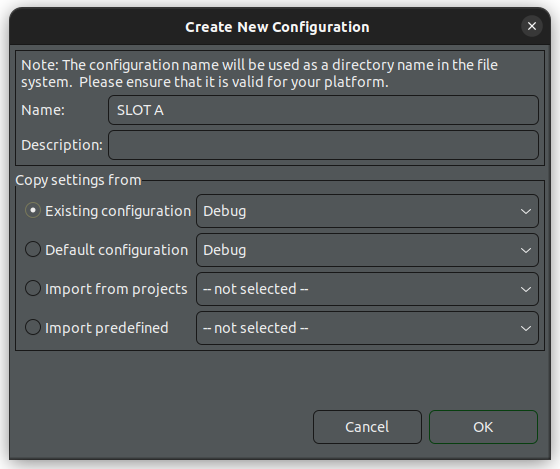
\includegraphics[width=0.6\textwidth]{res/stm32_new_build.png}
                \caption{Creando una nueva configuración de \emph{build}}
                \label{fig:stm32_new_build}
            \end{figure}

            A continuación, en las propiedades del proyecto, entramos a \texttt{C/C++ Build > Settings > MCU/MPU GCC Linker}. Tenemos que seleccionar arriba la configuración adecuada (A o B) y cambiar el nombre del \emph{linker script} al que acaba en \texttt{\_A} o \texttt{\_B} que hemos creado anteriormente. Esto se muestra en la \Cref{fig:stm32_build_setup}

            \begin{figure}
                \centering
                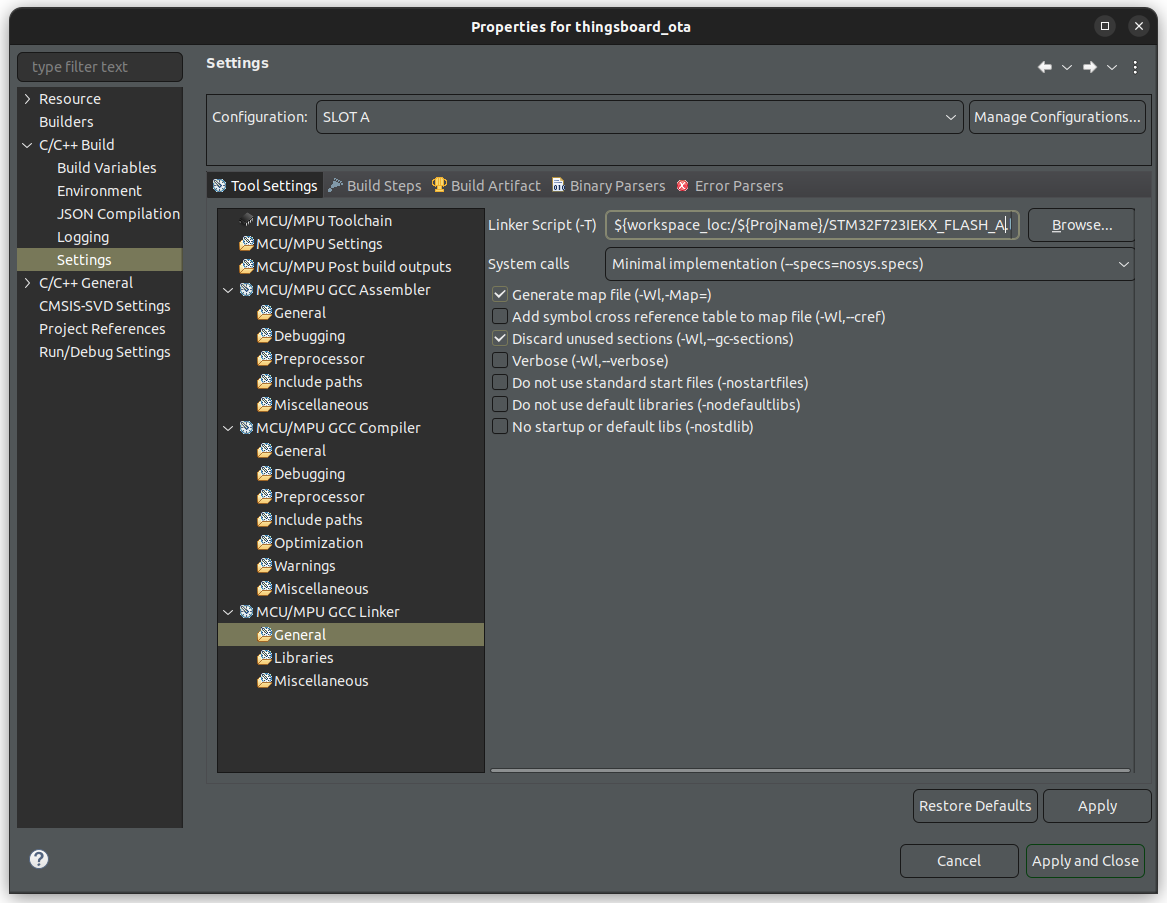
\includegraphics[width=0.8\textwidth]{res/stm32_build_setup.png}
                \caption{Configuración de linker script}
                \label{fig:stm32_build_setup}
            \end{figure}

            También debemos activar la opción de generar binario desde la misma configuración del proyecto, en \texttt{C/C++ Build > Settings > MCU/MPU Settings} (\Cref{fig:stm32_build_binary}).

            \begin{figure}
                \centering
                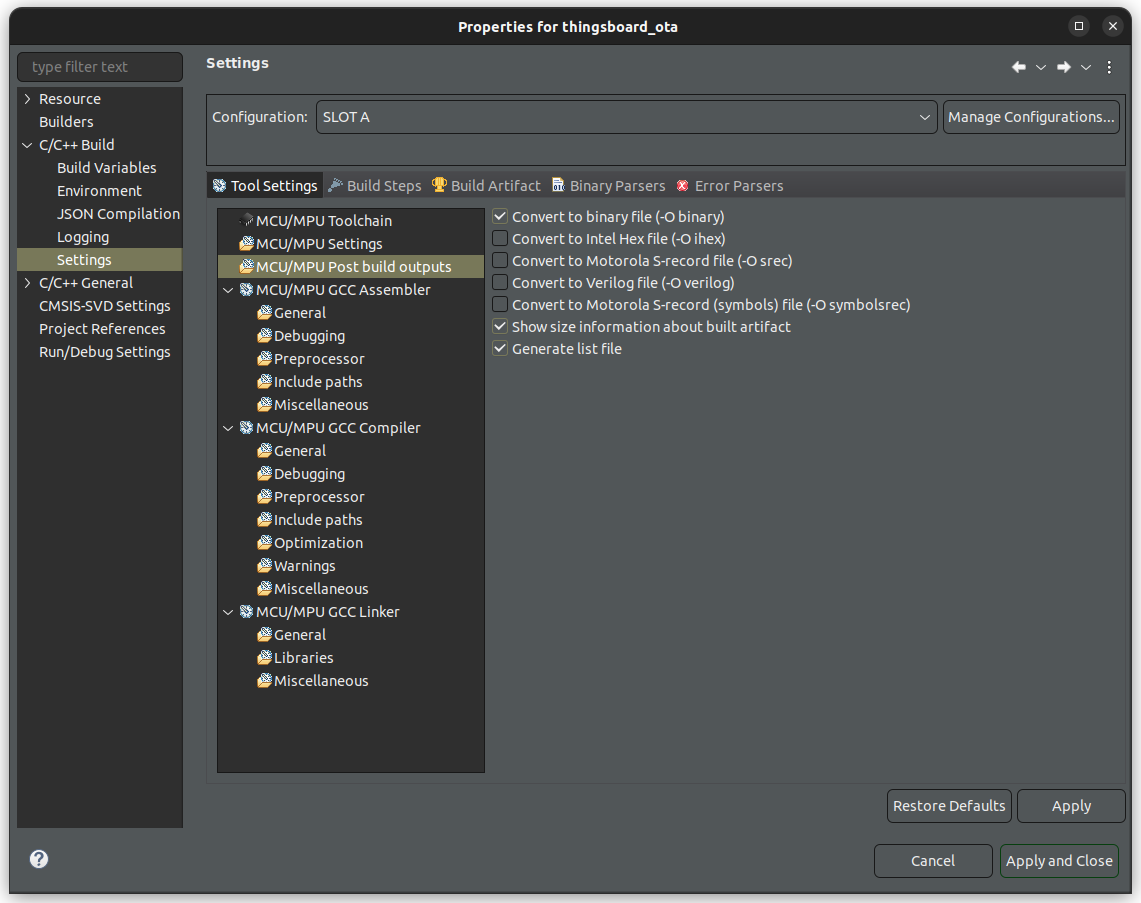
\includegraphics[width=0.8\textwidth]{res/stm32_build_binary.png}
                \caption{Configuración para generar archivo binario}
                \label{fig:stm32_build_binary}
            \end{figure}

            Ahora ya podemos compilar los dos binarios diferentes. Para ello basta darle al martillo de arriba, en la configuración ``SLOT A'' o ``SLOT B''. Veremos aparecer en nuestro proyecto dos carpetas, con sendos nombres, que contendrán los archivos compilados de cada una de las versiones. Para depurar, tendremos que ir a \texttt{Debug > Debug Configurations} y elegir el binario que queremos depurar como muestra la \Cref{fig:stm32_debug_ab}.

            \begin{figure}
                \centering
                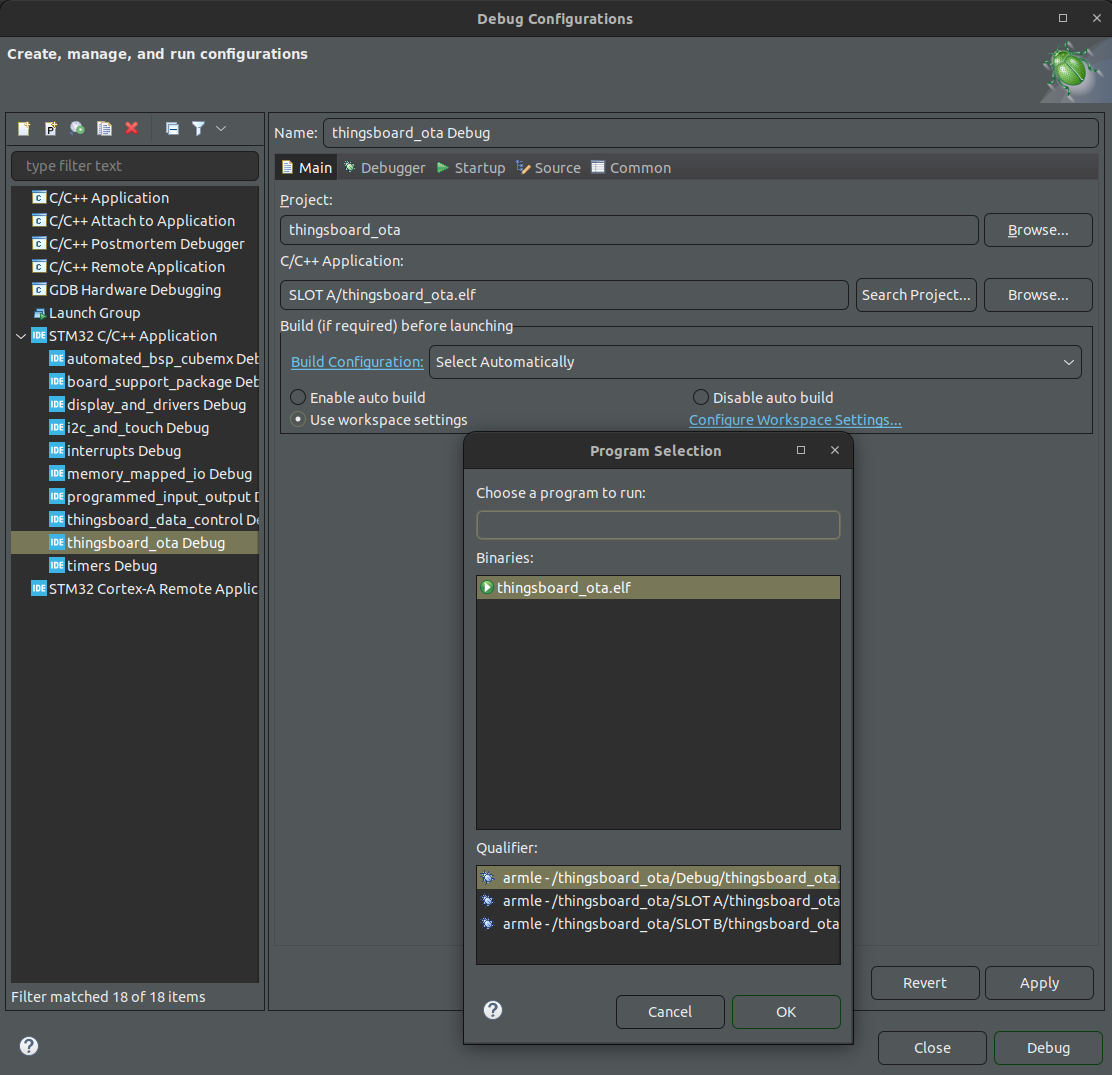
\includegraphics[width=0.8\textwidth]{res/stm32_debug_ab.png}
                \caption{Configuración para cambiar el binario de depuración}
                \label{fig:stm32_debug_ab}
            \end{figure}

            Al arrancar, deberíamos ver por terminal el siguiente mensaje, indicando que todo ha ido bien:

            \begin{lstlisting}
                [BOOT] Running App v1.0.0 from Address: 0x08000000
                [ESP] Testing ESP01S AT Communication...
                ...
            \end{lstlisting}

        \subsubsection{Configuración en \emph{Thingsboard}}

            Tras tener preparadas las dos compilaciones, podemos subirlas a \emph{ThingsBoard}. Para ello, hay que ir a la sección \texttt{Advanced Features > OTA Updates} y añadir dos nuevos paquetes de Firmware. Tendremos que indicar un nombre y versión, además de asociarlo con un perfil (por defecto en nuestro caso), y subir el binario. Todo el proceso se muestra en la \Cref{fig:thingsboard_ota_upload}

            \begin{figure}
                \centering
                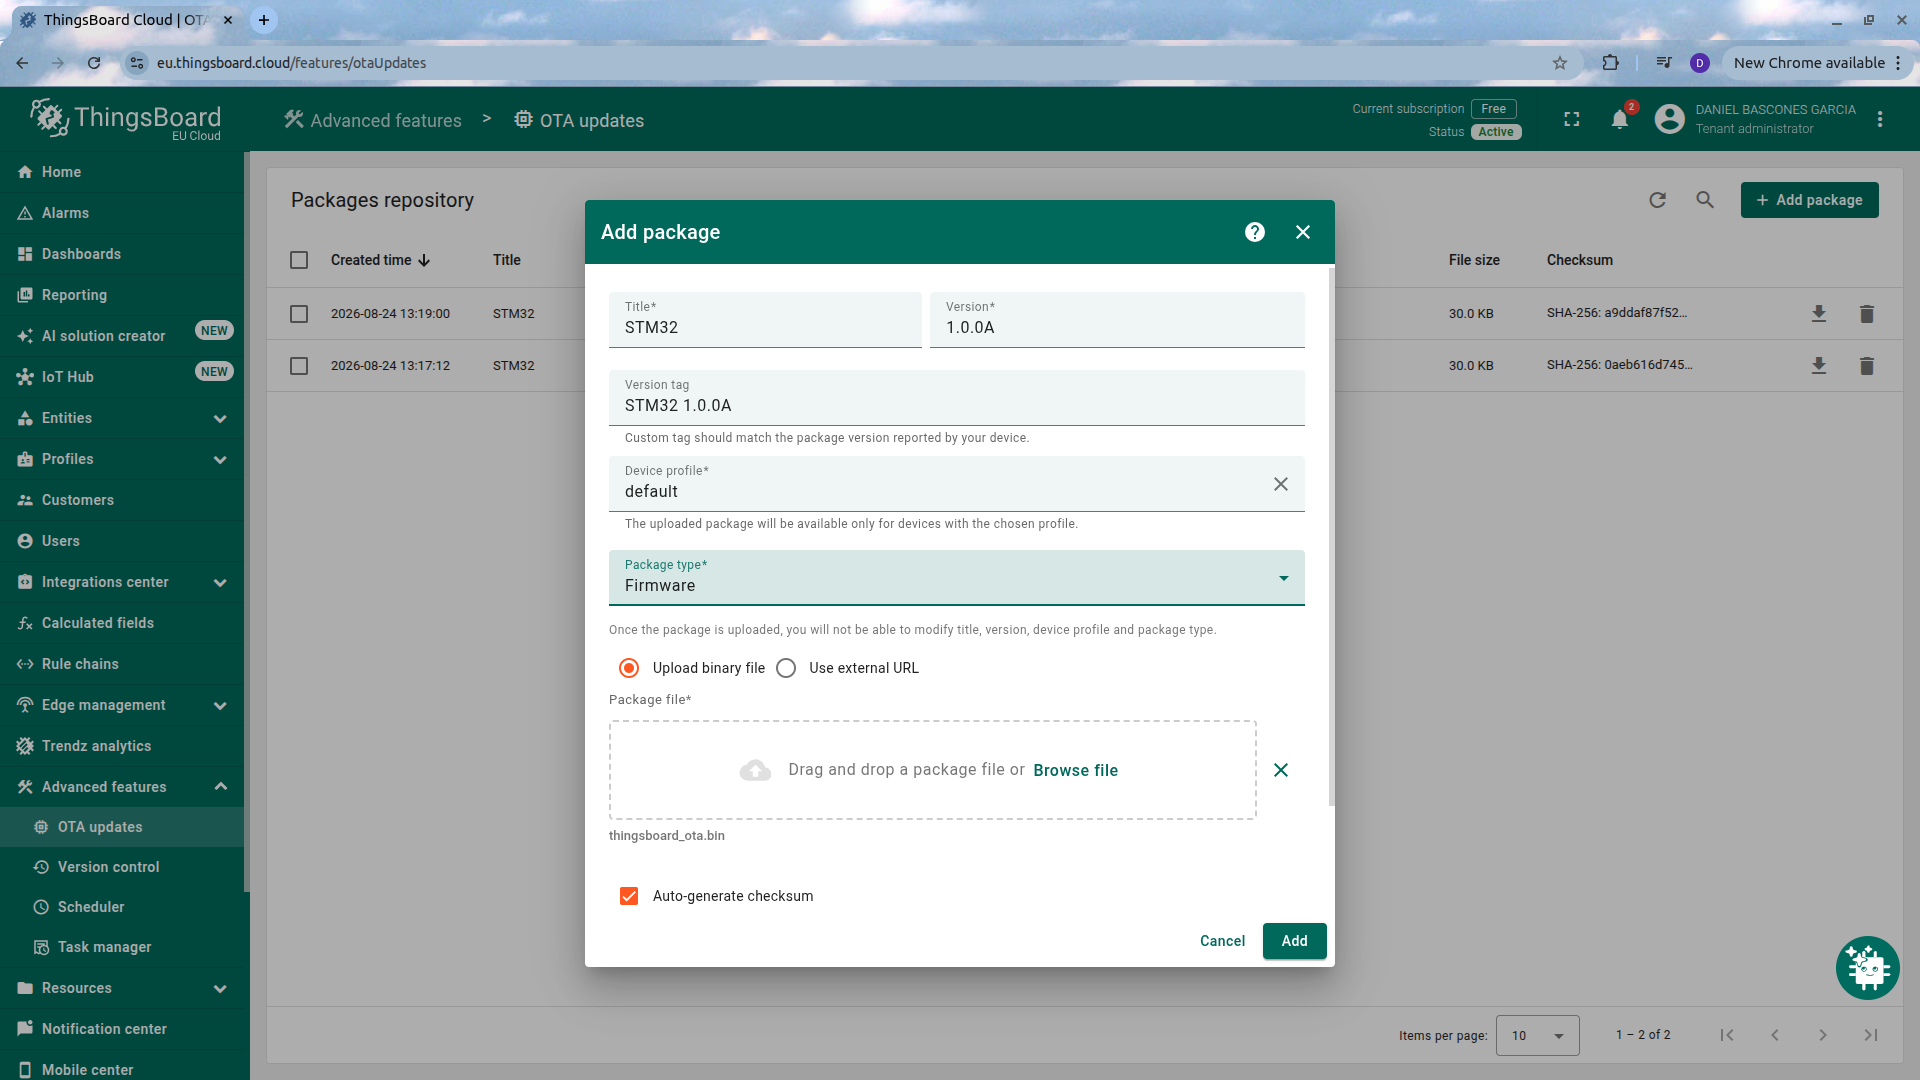
\includegraphics[width=\textwidth]{res/thingsboard_ota_upload.png}
                \caption{Subida de Firmware para OTA a \emph{ThingsBoard}}
                \label{fig:thingsboard_ota_upload}
            \end{figure}

            Podemos subir diferentes versiones, y seleccionar en cada momento la que nuestro dispositivo debería tener. En este caso, lo hacemos desde el apartado de \texttt{Entities > Devices}, donde podremos seleccionar, para nuestro dispositivo (ver \Cref{fig:thingsboard_ota_select}), el firmware que queramos y será anunciado mediante \textbf{MQTT}.

            \begin{figure}
                \centering
                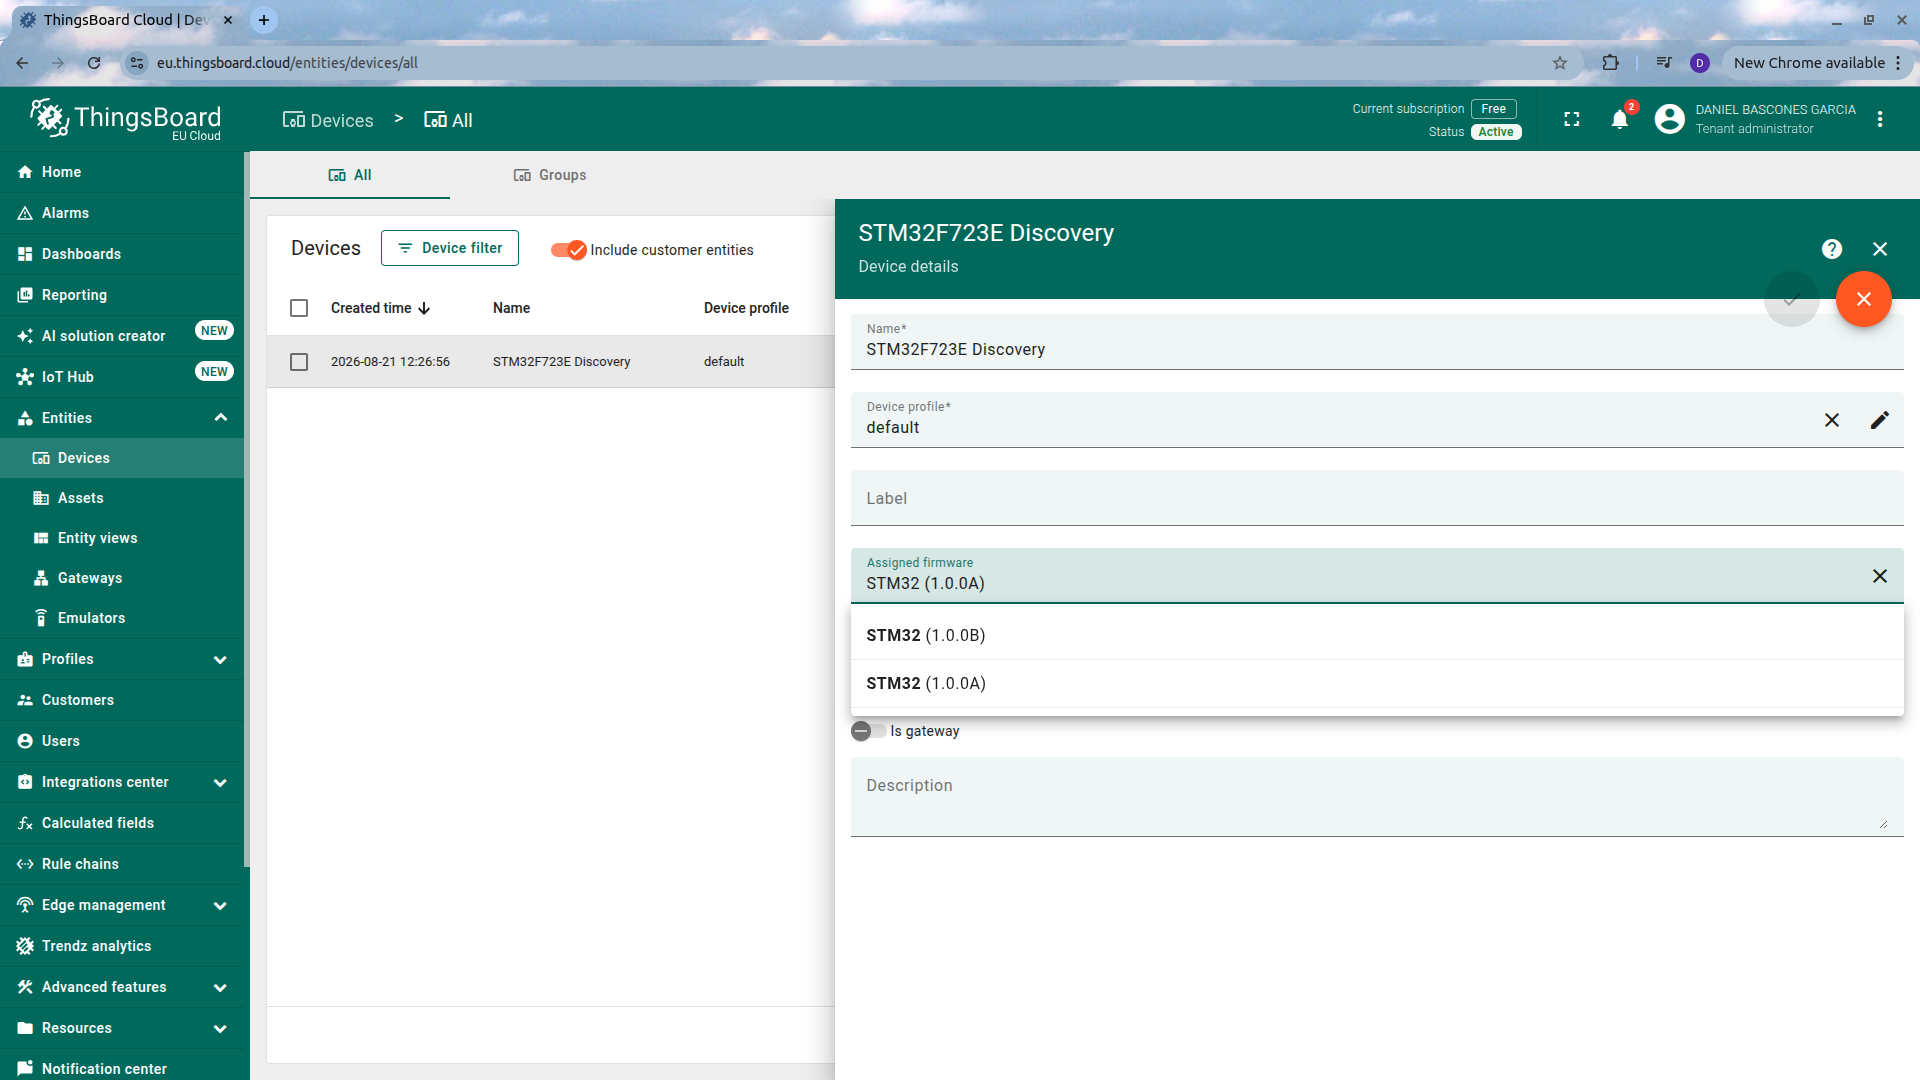
\includegraphics[width=\textwidth]{res/thingsboard_ota_select.png}
                \caption{Subida de Firmware para OTA a \emph{ThingsBoard}}
                \label{fig:thingsboard_ota_select}
            \end{figure}

            Por ejemplo, podemos seleccionar el firmware ``A'' (\texttt{Devices > Details > Assigned Firmware}) y arrancar la aplicación, desde STM32CubeIDE, también en el slot A. Si abrimos una terminal para ver los mensajes de depuración, deberíamos observar lo siguiente:

            \begin{lstlisting}
                [BOOT] Running App v1.0.0 from Address: 0x08000000
                [ESP] Testing ESP01S AT Communication...
                [ESP] Disabling Echo...
                [ESP] Setting Station Mode...
                [ESP] Disabling MUX (Single Conn Mode)...
                [ESP] Enabling Transparent Passthrough Mode...
                [ESP] Connecting to SSID: guayfi...
                [MQTT] Connecting to eu.thingsboard.cloud:1883...
                [MQTT] Entering passthrough streaming...
                [MQTT RX] CONNACK 0x00: Connection Accepted!
                [MQTT RX] SUBACK Received! Granted QoS: 0
                [MQTT] Connected & Subscribed successfully!
                [SYSTEM] Ready! Streaming over MQTT...
                [MQTT TX] {"temp":20.50,"counter":1,"touch_x":15,"touch_y":20}
                [OTA] Rejected update 1.0.0A! Device is running in Slot A and requires B binary.
            \end{lstlisting}

            Podemos ver que, como el firmware seleccionado es para el mismo Slot, la aplicación lo rechaza y no actualiza nada. Si lo hiciera, colocaría un código que asume su inicio en \MEMORY{0x08000000} en la dirección de B \MEMORY{0x08040000}, donde cualquier salto absoluto resultaría en un fallo de ejecución. Si a continuación cambiamos el firmware objetivo desde \emph{ThingsBoard} para nuestro dispositivo (\texttt{Devices > Details > Assigned Firmware}), la aplicación recibirá la actualización y, ahora sí, descargará la actualización:

            \begin{lstlisting}
                [OTA] New Version Found: 1.0.0B (Size: 18628 bytes)
                [OTA] Erasing Slot B (0x08040000)...
                [OTA] Target Slot Erased!
                [OTA RX] Chunk 1 (512 bytes) -> Total: 512 / 18628
                // .............. Descarga de actualización
                [OTA RX] Chunk 37 (196 bytes) -> Total: 18628 / 18628
                // .............. Cambio de arranque
                [OTA SUCCESS] Download Finished! Rebooting...
                [OTA] Swapping BOOT_ADD0 to 0x0000000U (val: 0x8040000) and resetting...
                // .............. Nuevo arranque desde SLOT B
                [BOOT] Running App v1.0.0 from Address: 0x08040000
                // .............. App en marcha! Ahora rechaza la aplicación nueva.
                [OTA] Rejected update 1.0.0B! Device is running in Slot B and requires A binary.
                [MQTT TX] {"temp":21.00,"counter":2,"touch_x":30,"touch_y":40}
            \end{lstlisting}

            Si volvemos a cambiar el Firmware por el A, la aplicación volverá a actualizarse gracias a los avisos que envía \emph{ThingsBoard} con cada cambio de versión.

    \subsection{Para hacer más}

        En nuestro caso, estamos descargando ``a ciegas'' la aplicación, grabándola en la \PER{FLASH}, y dándole el control con mucha confianza. Normalmente, al descargar una imagen binaria, también se envía un CRC o código de comprobación. Así, la aplicación puede calcular el CRC de los datos descargados, comprobarlo contra el CRC enviado por el servidor, y cambiar los bits de arranque únicamente si coinciden, asegurando la integridad de la app. Investiga cómo podría hacerse esto y qué cambios harían falta tanto en \emph{ThingsBoard} como en nuestro código fuente.

\end{document}